\synctex=1
\documentclass[11pt,aspectratio=169]{beamer}

\usepackage[T1]{fontenc}
\usepackage[english,provide=*]{babel}
\usepackage{amsmath,amssymb,amsfonts}
\usepackage{mathtools}
\usepackage{bm}
\usepackage{tikz}
\usetikzlibrary{arrows.meta,positioning,shapes,calc,decorations.pathreplacing}
\usepackage{pgfplots}
\usepackage{xcolor}
\usepackage{booktabs}
\pgfplotsset{compat=1.18}

\usefonttheme[onlymath]{serif}

\definecolor{darkblue}{RGB}{0,51,102}
\definecolor{lightblue}{RGB}{230,240,250}
\definecolor{darkgreen}{RGB}{0,102,51}
\definecolor{darkred}{RGB}{153,0,0}
\definecolor{orange}{RGB}{255,128,0}
\definecolor{violet}{RGB}{102,0,153}
\definecolor{lightgreen}{RGB}{220,245,220}
\definecolor{lightorange}{RGB}{255,240,220}
\definecolor{gray}{gray}{0.4}

% Git hash for the footer.
\usepackage{xstring}
\usepackage{catchfile}
\immediate\write18{git rev-parse HEAD > git.hash}
\CatchFileDef{\HEAD}{git.hash}{\endlinechar=-1}
\newcommand{\gitrevision}{\StrLeft{\HEAD}{7}}

\usepackage{ccicons}

\setbeamertemplate{footline}{
  \hfill\vspace*{1pt}\href{https://creativecommons.org/publicdomain/zero/1.0/deed.en}{\cczero}\enspace\href{https://github.com/stepan-a/continuo}{\gitrevision}\enspace--\enspace\insertframenumber/\inserttotalframenumber\enspace--\enspace\today\enspace}

\setbeamertemplate{navigation symbols}{}

\hypersetup{colorlinks=true}

\DeclareMathOperator*{\argmax}{arg\,max}
\DeclareMathOperator*{\argmin}{arg\,min}

\title{Solving continuous time perfect-foresight models}
\author{Stéphane Adjemian}
\institute{Université du Mans}

\AtBeginSection[]
{
  \begin{frame}
    \frametitle{Plan}
    \tableofcontents[currentsection]
  \end{frame}
}

\begin{document}

\begin{frame}
\titlepage
\end{frame}


\begin{frame}{Plan}
\tableofcontents
\end{frame}

%==============================================================================
\section{Perfect foresight in dynamic economics}
%==============================================================================

\begin{frame}{Perfect foresight -- What we are solving}

\begin{itemize}

\item Macro/finance models routinely produce systems of differential
  or difference equations mixing \textbf{predetermined states}
  (capital, debt, habit stock) and \textbf{forward-looking jumps}
  (consumption, inflation, asset prices, costates).\newline

\item Under \textbf{perfect foresight}, agents know the entire future
  path of exogenous variables. The model collapses to a
  \textbf{deterministic two-point boundary-value problem (BVP)}:\newline
  \begin{itemize}
  \item states are pinned at $t=0$ by their initial condition,\newline
  \item jumps are pinned far in the future by the terminal steady
    state (saddle-path stability).
  \end{itemize}

\medskip
  
\item The BVP is non-linear, typically has no closed form, and must be
  solved \textbf{numerically}: discretise (if time is continuous), then run Newton.

\end{itemize}

\end{frame}

\begin{frame}{Perfect foresight -- Why bother?}

\begin{itemize}

\item Perfect-foresight transitions are the workhorse for:\newline
  \begin{itemize}
  \item transition dynamics after a permanent policy change
    (Ramsey, fiscal reform),\newline
  \item the response to a pre-announced (anticipated) sequence
    of shocks,\newline
  \item occasionally-binding constraints (ZLB, borrowing limits)
    where local linearisation fails,\newline
  \item non-linear models where second-order Taylor expansions miss
    the action.
  \end{itemize}

\end{itemize}

\end{frame}

\begin{frame}{Perfect foresight -- Two flavours}

\begin{itemize}

\item \textbf{Discrete time} (Dynare's natural setting): the model is
  a system of non-linear equations
  \[
  f\bigl(y_{t+1},\,y_t,\,y_{t-1},\,u_t,\,\theta\bigr) \;=\; 0,
  \qquad t = 1, \ldots, T,
  \]
  with $y_0$ given (states) and $y_{T+1} = \bar y$
  (terminal steady state).\newline

\item \textbf{Continuous time} (Continuo's setting): the model
  is an implicit differential-algebraic equation (DAE)
  \[
  F\bigl(\dot x(t),\, x(t),\, e(t),\, \theta,\, t\bigr) \;=\; 0,
  \qquad t \in [0,T],
  \]
  with $x_S(0)$ given (states) and $x_J(T) = \bar x_J$ (jumps at the
  terminal steady state).\newline

\item Both reduce, after suitable discretisation, to a large
  block-sparse \textbf{non-linear} system solved by Newton. The
  difference lies in \emph{how} the time derivative is approximated.

\end{itemize}

\end{frame}

%==============================================================================
\section{Continuous-time setup}
%==============================================================================

\begin{frame}{Continuous time -- The model}

\begin{itemize}

\item The model is an implicit DAE on the horizon $[0,T]$:
  \[
  \boxed{F\bigl(\dot x,\, x,\, e,\, \theta,\, t\bigr) \;=\; 0,}
  \]
  $x\in\mathbb R^n$, $e\in\mathbb R^{n_e}$ exogenous,
  $\theta$ parameters. $F$ takes values in $\mathbb R^n$.\newline

\item Endogenous variables split into $n_S$ \textbf{states}, $n_J$ \textbf{jumps} (together: $n_d = n_S+n_J$
    \emph{dynamic} variables, the ones with a time derivative), and $n_a = n - n_d$ \textbf{algebraic} variables, defined by static
    relations.\newline

\item Equations split accordingly into $n_d$ \emph{dynamic rows}
  (depending on $\dot x$) and $n_a$ \emph{algebraic rows}
  (pure equalities). Continuo detects the partition
  automatically from CasADi's symbolic dependency graph.

\end{itemize}

\end{frame}

\begin{frame}{Continuous time -- Boundary conditions}

\begin{itemize}

\item \textbf{Initial condition (states).} Each state $x_s$ ($s\in S$)
  is pinned at $t=0$:
  \[
  x_s(0) \;=\; x_s^{0},
  \qquad s\in S.
  \]
  In Continuo these values come from the \texttt{initval}
  block (often the initial steady state).\newline

\item \textbf{Terminal condition (jumps).} Each jump $x_j$ ($j\in J$)
  is pinned at the \emph{terminal} steady state:
  \[
  x_j(T) \;=\; x_j^{\star},
  \qquad j\in J,
  \]
  computed at the exogenous belief $e(T)$.\newline

\item \textbf{Algebraic variables} need no boundary condition: their
  values are determined at every $t$ by the algebraic rows of $F$.\newline

\item Together, $n_S + n_J = n_d$ boundary conditions, matching the
  $n_d$ first-order differential equations. The BVP is well-posed.

\end{itemize}

\end{frame}

\begin{frame}{Continuous time -- Example: Ramsey--Cass--Koopmans}

\begin{itemize}

\item Felicity $u(c)=c^{1-\sigma}/(1-\sigma)$, technology $f(k)$,
  depreciation $\delta$, discount $\rho$, single exogenous TFP shifter
  $z$ entering $f$:
  \[
  \dot k \;=\; z\,f(k) - \delta k - c,
  \qquad
  \dot c \;=\; \tfrac{c}{\sigma}\bigl(z\,f'(k) - \delta - \rho\bigr).
  \]

\item State: $k$ (capital, predetermined). Jump: $c$
  (consumption, chosen at every $t$).\newline

\item Boundary conditions:
  \[
  k(0) = k_0,
  \qquad
  c(T) = \bar c\bigl(z(T)\bigr).
  \]

\item No algebraic variables here ($n_a=0$). In general Continuo
  handles $n_a>0$ transparently (intermediate definitions, market
  clearing, etc.).

\end{itemize}

\end{frame}

%==============================================================================
\section{From BVP to non-linear system}
%==============================================================================

\begin{frame}{Discretisation -- Strategy}

\begin{itemize}

\item Choose a grid on $[0,T]$ with $N$ intervals:
  \[
  0 = t_0 < t_1 < \cdots < t_N = T,
  \qquad
  dt = T/N,
  \quad
  t_{i+\frac12} = \tfrac12(t_i+t_{i+1}).
  \]

\item Replace the BVP by $N{+}1$ \emph{unknown vectors} $x_0,x_1,\ldots,x_N \in \mathbb R^n$,
  one per grid point, stacked into
  \[
  X \;=\; \bigl(x_0^\top, x_1^\top, \ldots, x_N^\top\bigr)^\top
  \;\in\; \mathbb R^{n(N+1)}.
  \]

\item Replace the differential equation by an \textbf{algebraic} link
  between consecutive points (\emph{collocation}), plus enforce the
  algebraic rows pointwise and the boundary conditions.\newline

\item Result: a square non-linear system $G(X)=0$ of size
  $n(N{+}1)$, solved by \textbf{Newton} with a sparse linear solver.

\end{itemize}

\end{frame}

\begin{frame}{Discretisation -- The grid}

\begin{center}
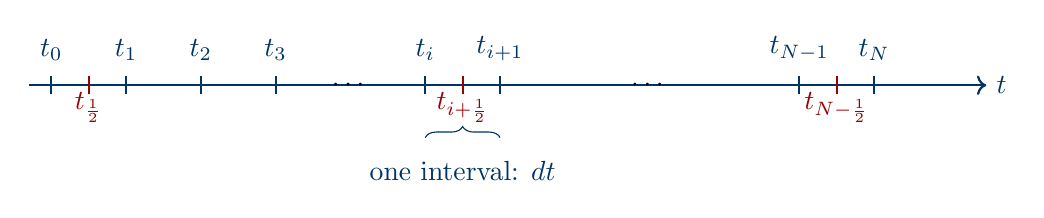
\begin{tikzpicture}[scale=0.95]
  \draw[->,thick,darkblue] (-0.3,0) -- (12.5,0) node[right] {$t$};
  \foreach \i/\lab in {0/$t_0$,1/$t_1$,2/$t_2$,3/$t_3$,5/$t_{i}$,6/$t_{i+1}$,10/$t_{N-1}$,11/$t_N$}
    \draw[thick,darkblue] (\i,-0.12) -- (\i,0.12) node[above=2pt] {\lab};
  \foreach \i/\lab in {0.5/$t_{\frac12}$,5.5/$t_{i+\frac12}$,10.5/$t_{N-\frac12}$}
    \draw[thick,darkred] (\i,-0.12) -- (\i,0.12) node[below=2pt,darkred] {\lab};
  \node at (4,0) {$\cdots$};
  \node at (8,0) {$\cdots$};

  \draw[decorate,decoration={brace,amplitude=4pt},darkblue]
    (5,-0.7) -- (6,-0.7) node[midway,below=5pt] {one interval: $dt$};
\end{tikzpicture}
\end{center}

\begin{itemize}

\item $N{+}1$ \textbf{grid points} $t_0,\ldots,t_N$ (blue): the
  unknowns $x_i \equiv x(t_i)$ live here.\newline

\item $N$ \textbf{midpoints} $t_{i+\frac12}$ (red): additional
  collocation points used by some schemes to evaluate the model
  inside each interval.\newline

\item By default a uniform grid between $0$ and $T$ is considered;  the spacing $dt$ is the
  same for every interval.

\end{itemize}

\end{frame}

%==============================================================================
\section{Approximating the exponential}
%==============================================================================

\begin{frame}{Approximation -- The one-step problem}

\begin{itemize}

\item A \textbf{one-step scheme} for $\dot x = g(x,t)$ produces
  $x_{i+1}$ from $x_i$ alone, possibly via internal evaluations of $g$
  inside $[t_i, t_{i+1}]$ but without referencing earlier
  $x_{i-1}, x_{i-2}, \ldots$ (as multistep methods would do).\newline

  \item Such a scheme is judged by how well one step approximates the
  exact \textbf{flow map} $x(t_{i+1}) = \Phi_{dt}\bigl(x(t_i)\bigr)$:
  consistency, accuracy, stability all reduce to how close the
  scheme's update is to $\Phi_{dt}$.\newline

\item As we will demonstrate below, $\Phi_{dt}$ can be constructed
  straightforwardly when the exact solution to the differential
  equation is available.\newline

\item We will focus on the first-order linear homogeneous ordinary
  differential equation.\newline

\end{itemize}

\end{frame}

\begin{frame}{Approximation -- A simple test problem}

\begin{itemize}

\item We consider the simplest ODE:
  \[
    \dot x = \lambda\, x
  \]
  with $\lambda\in\mathbb C$, $x(0)=1$. The exact solution $x(t)=e^{\lambda t}$ converges to 0 iff $\mathrm{Re}(\lambda)<0$.\newline

\item Every one-step scheme applied to the test problem produces an
  iterate of the form $x_{i+1} = A(\lambda\, dt)\, x_i$. The
  \textbf{amplification factor} $A(z)$, $z=\lambda\, dt$, is the
  scheme's approximation of $e^z$. Two fundamental questions:\newline
  \begin{itemize}
  \item \emph{Accuracy.} How many Taylor coefficients of $e^z$ does
    $A$ get right?\newline
  \item \emph{Stability.} Is $|A(z)|\le 1$ on the left half-plane
    $\mathrm{Re}(z)<0$?
  \end{itemize}

  \medskip

\item \textbf{Conditionally stable}: $|A|\le 1$ only for $dt$ below
  some $\lambda$-dependent threshold. \textbf{A-stable}: $|A|\le 1$
  for every $z$ with $\mathrm{Re}(z)<0$. \textbf{L-stable}: A-stable
  \emph{and} $|A(z)|\to 0$ as $\mathrm{Re}(z)\to-\infty$
  (cf.\ next slide).

\end{itemize}

\end{frame}

\begin{frame}{Approximation -- A-stable vs.\ L-stable}

\begin{itemize}

\item A-stability prevents blow-up but says nothing about damping:
  for $|\lambda\, dt|$ very large $e^{\lambda dt}\approx 0$, yet
  $|A(\lambda dt)|$ may sit near $1$ — and when $A\approx -1$ the
  iterate flips sign at every step ($+,-,+,-$ at amplitude $\sim\!1$):
  a parasitic sawtooth, while the true solution decays monotonically.
  \textbf{L-stability} adds $|A(z)|\to 0$ as $|z|\to\infty$ on the
  left half-plane, killing fast modes in one step.\newline

\item Two representative rational $A(z)$ at $\lambda\, dt = -100$:
  \begin{center}
    \scriptsize
    \renewcommand{\arraystretch}{1.3}
    \begin{tabular}{lccl}
      \toprule
      $A(z)$ & type & $A(-100)$ & after one step \\
      \midrule
      $(1+z/2)/(1-z/2)$ & A-stable, not L &
        $(1{-}50)/(1{+}50) \approx -0.96$ &
        sawtooth at amplitude $\sim\!1$ \\
      $1/(1-z)$ & L-stable &
        $1/(1{+}100) \approx 0.01$ &
        damped to $\sim 0$ \\
      $e^z$ (exact) & — & $\sim 10^{-44}$ & essentially zero \\
      \bottomrule
    \end{tabular}
  \end{center}

\medskip
  
\item This matters in \emph{multivariate} problems whose Jacobian has
  eigenvalues of widely different magnitudes — the standard notion of
  \textbf{stiffness}. Usually, A-stability suffices for
  perfect-foresight macro. L-stability is mentioned only because the
  Padé catalogue (next section) will classify some schemes as such.

\end{itemize}

\end{frame}

\begin{frame}{Approximation -- Local vs.\ global error}

\begin{itemize}

\item \textbf{Local error} (per step). Assume $x_i = x(t_i)$ exactly,
  apply the scheme once:
  $e_i^{\text{loc}} = x_{i+1}^{\text{scheme}} - x(t_{i+1})$ — the
  error from a \emph{single} step, starting from the truth.\newline

\item \textbf{Global error} at horizon $T$. Run the scheme from $t_0
  = 0$ to $t_N = T$ with $N = T/dt$ steps:
  $e^{\text{glob}}(T) = x_N^{\text{scheme}} - x(T)$.\newline

\item \textbf{Order.} A scheme is of \emph{global order} $p$ if
  $e_i^{\text{loc}} = O(dt^{p+1})$. Summing over $N = T/dt$ steps,
  \[
  e^{\text{glob}}(T) \;=\; \underbrace{O(T/dt)}_{N\,\sim\,1/dt}\cdot O(dt^{p+1})
  \;=\; T\cdot O\!\bigl(dt^{p+1}/dt\bigr) \;=\; O(dt^p)
  \]
  the $1/dt$ (more steps) cancels exactly one power of $dt$.
  Local order $=$ global order $+ 1$. When these slides say "scheme
  of order $p$", they mean \emph{global} order $p$.\newline

\item \textbf{Caveat.} The stacking $N\times e^{\text{loc}}$ requires
  the scheme to be \emph{stable}; otherwise local errors amplify
  exponentially.

\end{itemize}

\end{frame}

\begin{frame}{Why is the simplest ODE of interest? -- Nonlinear scalar problems}

\begin{itemize}

\item For $\dot x = g(x,t)$, $x\in\mathbb R$, linearise around
  $(x_i,t_i)$. With $\delta = x - x_i$, $\lambda_i = g'(x_i,t_i)$,
  $g_i = g(x_i,t_i)$ (constant over one step):
  $\dot\delta = \lambda_i\,\delta + g_i$, $\delta(0)=0$.\newline

\item Multiply by $e^{-\lambda_i t}$ so
  $\tfrac{d}{dt}\bigl(e^{-\lambda_i t}\delta\bigr) = g_i\,e^{-\lambda_i t}$;
  integrate $t$ from $0$ to $dt$:
  \[
  \delta(dt) \;=\; g_i\,\frac{e^{\lambda_i\, dt}-1}{\lambda_i}
  \;=\; dt\,g_i + \tfrac{dt^2}{2}\lambda_i g_i + O(dt^3).
  \]

\item \textbf{Forward Euler}, $x_{i+1} = x_i + dt\,g(x_i,t_i)$, on the
  nonlinear ODE reproduces only $dt\,g_i$ — local error
  $\tfrac{dt^2}{2}\lambda_i g_i = O(dt^2)$, hence \textbf{global order 1}.
  The same order emerges from the test problem $\dot x = \lambda x$:
  FE gives $x_{i+1} = x_i + \lambda\,x_i\,dt = (1+\lambda\,dt)\,x_i$, defining its
  \textbf{amplification factor} $A_{\mathrm{FE}}(z) = 1+z$ ($z = \lambda\,dt$).
  Compared to $e^z = 1+z+z^2/2+\cdots$, the gap is
  $A_{\mathrm{FE}}(z) - e^z = -z^2/2 + O(z^3)$ — local error $O(dt^2)$,
  global order 1, matching the nonlinear ODE. \textbf{General rule}:
  a scheme's global order $p$ on any smooth ODE equals the order at
  which $A(z) - e^z = O(z^{p+1})$ at $z=0$.

\end{itemize}

\end{frame}

\begin{frame}{Why is the simplest ODE of interest? -- Forced linear scalar problems}

\begin{itemize}

\item For $\dot x = \mu x + u(t)$, $x\in\mathbb R$, with anticipated
  forcing $u(t)$, variation of parameters gives the exact one-step
  \[
  x(t_{i+1}) \;=\; e^{\mu\, dt}\, x(t_i)
  \;+\; \int_{t_i}^{t_{i+1}} e^{\mu(t_{i+1}-s)}\, u(s)\, ds.
  \]

\item Applying forward Euler:
  \[
  x_{i+1} \;=\; x_i + dt\bigl(\mu x_i + u(t_i)\bigr)
  \;=\; \underbrace{(1+\mu\, dt)}_{A_{\mathrm{FE}}(\mu\, dt)}\, x_i
  \;+\; \underbrace{dt\, u(t_i)}_{\approx\,\int e^{\mu(\cdot)}u\,ds}.
  \]
  The $dt\,u(t_i)$ piece approximates the \emph{full} kernel-weighted
  integral: for small $dt$ both $e^{\mu(t_{i+1}-s)}\to 1$ and
  $u(s)\to u(t_i)$, leaving an $O(dt^2)$ remainder. Together with the
  $O(dt^2)$ homogeneous gap, FE is \textbf{global order 1}.\newline

\item General pattern: every one-step scheme gives
  $x_{i+1} = A(\mu\,dt)\,x_i +$ (weighted sum of $u$-samples). Net
  global order $= \min(p, q)$, with $p$ from $A(z) - e^z = O(z^{p+1})$
  and $q$ the order of the scheme's \emph{quadrature rule} on $u$.

\end{itemize}

\end{frame}

\begin{frame}{Why is the simplest ODE of interest? -- Nonlinear with forcing}

\begin{itemize}

\item General scalar problem $\dot x = g(x, u(t), t)$. Linearise around
  $(x_i, t_i)$ with $\delta = x - x_i$, $\lambda_i = \partial_x g$,
  $\beta_i = \partial_u g$, $g_i = g(x_i, u(t_i), t_i)$:
  \[
  \dot\delta \;\approx\; \lambda_i\,\delta \;+\; g_i
  \;+\; \beta_i\,\bigl[u(t) - u(t_i)\bigr]
  \]
  — a linear ODE with constant drift $g_i$ \emph{and} time-varying
  forcing, combining the two preceding scenarios.\newline

\item Variation of parameters splits the exact one-step into three
  pieces: homogeneous propagator $e^{\lambda_i\, dt}$ (approximated
  by $A(z)$); constant-drift contribution $g_i\,(e^{\lambda_i\, dt}{-}1)/\lambda_i$
  (reproduced by every consistent scheme via $dt\,g_i$); time-varying
  forcing integral (discretised by the scheme's quadrature on $u$).\newline

\item Net \emph{global} order = $\min(p, q)$, where $p$ comes from
  $A(z) - e^z = O(z^{p+1})$ on the homogeneous side and $q$ is the
  order of the scheme's embedded \emph{quadrature rule} on $u$
  ($q=1$ for endpoint sampling, $q=2$ for trapezoidal/midpoint,
  higher for richer rules). \textbf{No new analysis required.}

\end{itemize}

\end{frame}

\begin{frame}{Padé -- General principle}

\begin{itemize}

\item For any function $f$ analytic near $0$ with Taylor series
  $f(z) = \sum_{k\ge 0} c_k\, z^k$, the \textbf{Padé approximant}
  $R_{p,q}$ of type $(p,q)$ is the unique rational function
  $R_{p,q}(z) = P_p(z)/Q_q(z)$ with $\deg P_p \le p$, $\deg Q_q \le q$,
  $Q_q(0)=1$, matching $f$ to order $p+q$:
  \[
  R_{p,q}(z) - f(z) \;=\; O\bigl(z^{p+q+1}\bigr).
  \]

\item The $q=0$ row recovers Taylor polynomials — Padé strictly
  generalises polynomial approximation.\newline

\item \textbf{Why rationals?} A rational function captures features
  no polynomial of finite degree can: \emph{poles} (e.g.\ $1/(1-z)$
  blows up at $z=1$) and \emph{boundedness at infinity}. Same logic
  as transfer functions and rational kernels in time-series
  analysis.\newline

\item \textbf{When?} Whenever we want maximum information from a fixed
  amount of local Taylor data — convergence acceleration, special
  functions, model-order reduction, integrators for ODEs.

\end{itemize}

\end{frame}

\begin{frame}{Padé -- Construction and an illustration on $\log(1+z)$}

\begin{itemize}

\item Multiplying out, $Q_q(z)\,f(z) - P_p(z) = O(z^{p+q+1})$.
  Matching coefficients of $z^0,\ldots,z^{p+q}$ gives a linear
  system: $q$ equations (orders $p{+}1,\ldots,p{+}q$) determine $Q_q$
  uniquely, then $p{+}1$ equations cascade to give $P_p$.\newline

\item \textbf{Illustration: $f(z) = \log(1+z)$}, $c_k = (-1)^{k-1}/k$:
  \[
  R_{1,0}(z) = z,
  \qquad
  R_{1,1}(z) = \frac{z}{1+z/2},
  \qquad
  R_{2,2}(z) = \frac{z + z^2/2}{1 + z + z^2/6}.
  \]
  At $z=1$, $\log 2 \approx 0.6931$:
  \begin{center}
    \scriptsize
    \renewcommand{\arraystretch}{1.25}
    \begin{tabular}{lccc}
      \toprule
      Approximant & Coeffs used & Value at $z=1$ & Error \\
      \midrule
      Taylor $z - z^2/2$ ($R_{2,0}$) & 2 & $0.5000$ & $-0.193$ \\
      Padé $R_{1,1} = z/(1+z/2)$  & 2 & $0.6667$ & $-0.027$ \\
      Padé $R_{2,2}$              & 4 & $0.6923$ & $-0.0008$ \\
      \bottomrule
    \end{tabular}
  \end{center}

\item Same Taylor information, the rational form is one to two orders
  of magnitude more accurate. Diagonal $(p,p)$ Padé converges
  quadratically in the order, vs.\ linearly for Taylor: \emph{more
  accuracy for the same data}.

\end{itemize}

\end{frame}

\begin{frame}{Padé -- Specialisation to $e^z$}

\begin{itemize}

\item For $f(z) = e^z$, $c_k = 1/k!$, the Padé system has a closed
  form $R_{p,q}(z) = \big[\sum_{k=0}^{p}\binom{p}{k}\tfrac{(p+q-k)!}{(p+q)!}z^k\big] \big/ \big[\sum_{k=0}^{q}\binom{q}{k}\tfrac{(p+q-k)!}{(p+q)!}(-z)^k\big]$.\newline

\item The first few entries of the \textbf{Padé table}:
  \begin{center}
    \scriptsize
    \renewcommand{\arraystretch}{1.4}
    \begin{tabular}{c|ccc}
      \toprule
       & $q=0$ & $q=1$ & $q=2$ \\
      \midrule
      $p=0$ & $1$ & $\tfrac{1}{1-z}$ & $\tfrac{1}{1-z+z^2/2}$ \\
      $p=1$ & $1+z$ & $\tfrac{1+z/2}{1-z/2}$ & $\tfrac{1+z/3}{1-2z/3+z^2/6}$ \\
      $p=2$ & $1+z+\tfrac{z^2}{2}$ & $\tfrac{1+2z/3+z^2/6}{1-z/3}$ &
              $\tfrac{1+z/2+z^2/12}{1-z/2+z^2/12}$ \\
      \bottomrule
    \end{tabular}
  \end{center}

  \medskip
  
  % Ehle (1969) -> https://cs.uwaterloo.ca/research/tr/1969/CS-RR-2010.pdf
\item[$\Rightarrow$] $R_{p,q}$ is A-stable iff $q\ge p$,
  L-stable iff $q>p$.

\end{itemize}

\end{frame}

\begin{frame}{Padé -- A catalogue of numerical schemes}

\begin{itemize}

\item Each Padé entry of $e^z$ \emph{is} a one-step scheme for the
  test problem — and, after $z\mapsto M\, dt$, for any linear system:
  \begin{center}
    \scriptsize
    \renewcommand{\arraystretch}{1.2}
    \begin{tabular}{lll}
      \toprule
      Padé entry & Scheme & Global order / stability \\
      \midrule
      $(1,0)$       & Forward Euler                              & $1$, conditional \\
      $(0,1)$       & Backward Euler                             & $1$, A- \& L-stable \\
      $(1,1)$       & \textbf{Crank--Nicolson} / impl.\ midpoint & $2$, A-stable \\
      $(s,s)$       & Gauss--Legendre IRK ($s$ stages)           & $2s$, A-stable \\
      $(s{-}1,s)$   & Radau IIA ($s$ stages)                     & $2s{-}1$, L-stable \\
      \bottomrule
    \end{tabular}
  \end{center}

\medskip
  
\item \textbf{Why $(1,1)$ for Continuo.} The smallest A-stable
  Padé approximant of $e^z$ that is also second-order. One implicit
  solve per step — same cost as backward Euler — for one extra order
  of accuracy. Higher entries need multiple internal stages; Radau IIA
  wins on stiff problems and is a planned alternative.

\end{itemize}

\end{frame}

%==============================================================================
\section{The Crank--Nicolson scheme}
%==============================================================================

\begin{frame}{Crank--Nicolson -- The implicit midpoint formula}

\begin{itemize}

\item The $(1,1)$-Padé approximant of $e^z$ is $R_{1,1}(z) =
  (1+z/2)/(1-z/2)$. Applied to the test problem $\dot x = \lambda x$,
  $(1-\lambda dt/2)\,x_{i+1} = (1+\lambda dt/2)\,x_i$, re-arranged as
  a finite-difference equation:
  \[
  \boxed{\;
  \frac{x_{i+1}-x_i}{dt}
  \;=\;
  \lambda\,\tfrac12(x_i + x_{i+1}).
  \;}
  \]

\item For a general right-hand side $\dot x = g(x,t)$ there are two
  equivalent realisations of the same $(1,1)$-Padé: the
  \textbf{trapezoidal rule} $\tfrac{x_{i+1}-x_i}{dt} = \tfrac12\bigl[g(x_i,t_i)+g(x_{i+1},t_{i+1})\bigr]$
  (the average of forward Euler $x_{i+1} = x_i + dt\,g(x_i,t_i)$ and
  backward Euler $x_{i+1} = x_i + dt\,g(x_{i+1},t_{i+1})$) and the
  \textbf{implicit midpoint rule}
  $\tfrac{x_{i+1}-x_i}{dt} = g\!\bigl(\tfrac{x_i+x_{i+1}}{2},\,
  t_{i+\frac12}\bigr)$ (evaluation at the midpoint).\newline

\item The two coincide on linear problems and to leading order on
  smooth nonlinear ones. Continuo uses the implicit midpoint
  form: one residual evaluation per interval, and the natural
  realisation for implicit DAEs.

\end{itemize}

\end{frame}

\begin{frame}{Crank--Nicolson -- Properties (summary)}

\begin{itemize}

\item \textbf{Second-order accurate.} Local truncation $O(dt^3)$,
  global error $O(dt^2)$. Halving $dt$ divides the error by $\sim 4$.\newline

\item \textbf{A-stable.} $|A(z)|\le 1$ on the whole left half-plane:
  stable for any $dt>0$. The user picks $dt$ for accuracy alone.\newline

\item \textbf{Symmetric in time.} $A(z)A(-z)=1$ on linear problems:
  reversing time and re-integrating recovers the same iterate
  exactly. No time direction is favoured — fitting for a BVP pinned
  from both the past (states) and the future (jumps).\newline

\item \textbf{Implicit.} One linear (or, for non-linear models,
  Newton-solved) system per step. In a BVP solve, all steps are
  coupled anyway — no extra cost.\newline

\item \textbf{Not L-stable.} $|A(z)|\to 1$ as $|z|\to\infty$ along
  the negative real axis: very stiff modes are damped only slowly.
  For genuinely stiff problems Radau IIA is preferable.

\end{itemize}

\end{frame}

\begin{frame}{Crank--Nicolson -- For implicit DAEs}

\begin{itemize}

\item Continuo's model is implicit: $F(\dot x,x,e,\theta,t)=0$.
  The Crank--Nicolson realisation on $[t_i,t_{i+1}]$ takes:
  \[
  \dot x \;\leftarrow\; \frac{x_{i+1}-x_i}{dt}
  \quad\text{(applied only to dynamic components)},
  \]
  \[
  x \;\leftarrow\; \tfrac12(x_i+x_{i+1}),
  \qquad
  e \;\leftarrow\; e(t_{i+\frac12}),
  \qquad
  t \;\leftarrow\; t_{i+\frac12}.
  \]

\item The per-interval residual is therefore
  \[
  R_i(x_i,x_{i+1})
  \;=\;
  F\!\left(\frac{x_{i+1}^d-x_i^d}{dt},\;
           \tfrac{x_i+x_{i+1}}{2},\;
           e(t_{i+\frac12}),\;\theta,\;
           t_{i+\frac12}\right),
  \]
  where $x^d$ collects the $n_d$ dynamic components.\newline

\item Implemented in \texttt{src/continuo/solve/disc/crank\_nicolson.py};
  built as a CasADi \texttt{Function} once, then evaluated symbolically
  at every interval when assembling the stacked system.

\end{itemize}

\end{frame}

%==============================================================================
\section{Worked examples}
%==============================================================================

\begin{frame}{Example -- A scalar ODE we can solve by hand}

\begin{itemize}

\item Consider the simplest linear stable ODE,
  \[
  \dot x \;=\; -\lambda x,
  \qquad x(0) = x_0,
  \qquad \lambda > 0.
  \]
  Exact solution: $x(t) = x_0 e^{-\lambda t}$.\newline

\item This is the linearisation of any stable economic relation
  around a steady state (the eigenvalue $-\lambda$ sets the speed of
  convergence). Here it has \emph{one} state, \emph{no} jump, so we
  drop the terminal condition.\newline

\item \textbf{Plan.} Apply the three schemes — forward Euler,
  backward Euler, Crank--Nicolson — on a uniform grid with step
  $dt = T/N$, derive each amplification factor, expose the defects
  of the two Eulers, and only then compare numerically.

\end{itemize}

\end{frame}

\begin{frame}{Example -- Forward Euler and its defects}

\begin{itemize}

\item Apply $x_{i+1} = x_i + dt\cdot g(x_i,t_i)$ with $g(x)=-\lambda x$:
  \[
  \boxed{\;x_{i+1} \;=\; (1 - \lambda\,dt)\,x_i,\qquad A_{\mathrm{FE}}(z) = 1+z,\quad z=-\lambda\,dt.\;}
  \]

\item \textbf{Accuracy.} Compare to $e^{-\lambda dt} = 1 - \lambda dt
  + \tfrac12(\lambda dt)^2 + O\bigl((\lambda dt)^3\bigr)$: the
  $(\lambda dt)^2$ term is missing entirely. Local error per step
  $\tfrac12(\lambda dt)^2 x_i = O(dt^2)$, hence \textbf{global order 1}.\newline

\item \textbf{Stability.} $|A_{\mathrm{FE}}| < 1 \iff 0 < \lambda dt
  < 2$: \emph{conditional} stability with the CFL-type bound $dt <
  2/\lambda$. Beyond it the iterate diverges.\newline

\item \textbf{Qualitative failure modes.}
  \begin{itemize}
  \item $\lambda dt = 1$: $A=0$, the iterate collapses to $x=0$ after
    one step (technically stable, but useless),
  \item $1 < \lambda dt < 2$: $A < 0$, the iterate \emph{oscillates}
    around zero — the true solution is monotonic,
  \item $\lambda dt = 2$: $A = -1$, sustained oscillation at constant
    amplitude (marginally stable),
  \item $\lambda dt > 2$: $A < -1$, divergence.
  \end{itemize}

\end{itemize}

\end{frame}

\begin{frame}{Example -- Backward Euler and its defects}

\begin{itemize}

\item Apply $x_{i+1} = x_i + dt\cdot g(x_{i+1},t_{i+1})$, again with
  $g(x)=-\lambda x$. Solve the implicit equation $(1+\lambda dt)\,x_{i+1} = x_i$:
  \[
  \boxed{\;x_{i+1} \;=\; \frac{1}{1+\lambda\,dt}\,x_i,\qquad A_{\mathrm{BE}}(z) = \frac{1}{1-z},\quad z=-\lambda\,dt.\;}
  \]

\item \textbf{Accuracy.} Expand $\tfrac{1}{1+\lambda dt} = 1 - \lambda
  dt + (\lambda dt)^2 - \cdots$. Coefficient on $(\lambda dt)^2$ is
  $1$, not $\tfrac12$: local error $\tfrac12(\lambda dt)^2 x_i = O(dt^2)$
  (opposite sign to FE — BE \emph{overestimates}), so again
  \textbf{global order 1}.\newline

\item \textbf{Stability.} $0 < A_{\mathrm{BE}} < 1$ for any $\lambda
  dt > 0$: A-stable, monotonic decay, no $dt$ restriction. \emph{No
  qualitative failure mode}, unlike FE.\newline

\item \textbf{Default.} As $\lambda dt \to \infty$, $A_{\mathrm{BE}}
  \to 0$ (BE is also L-stable). Fast modes are damped too aggressively
  — fine for genuinely stiff problems, but on smooth
  macro dynamics this kills information the user may want to see. And
  the price (implicit solve per step) buys only first-order accuracy.

\end{itemize}

\end{frame}

\begin{frame}{Example -- Crank--Nicolson on this problem}

\begin{itemize}

\item Same model in implicit DAE form: $F(\dot x, x) = \dot x +
  \lambda x = 0$. One dynamic row, no algebraic row. Per-interval
  residual on $[t_i, t_{i+1}]$:
  \[
  R_i(x_i,x_{i+1})
  \;=\;
  \underbrace{\frac{x_{i+1}-x_i}{dt}}_{\text{discrete }\dot x}
  \;+\;
  \lambda\,\underbrace{\tfrac12(x_i+x_{i+1})}_{\text{midpoint }x}
  \;=\; 0.
  \]

\item Setting $R_i = 0$ and isolating $x_{i+1}$:
  \[
  \boxed{\;
  x_{i+1} \;=\; \frac{1 - \tfrac12\,\lambda\, dt}{1 + \tfrac12\,\lambda\, dt}\,x_i,
  \qquad
  A_{\mathrm{CN}}(z) \;=\; \frac{1+z/2}{1-z/2}.
  \;}
  \]

\item Taylor-expand: $A_{\mathrm{CN}}(-\lambda dt) = 1 - \lambda dt +
  \tfrac12(\lambda dt)^2 - \tfrac14(\lambda dt)^3 + \cdots$ — matches
  $e^{-\lambda dt}$ through the $(\lambda dt)^2$ term, so the local
  error per step is $\bigl(\tfrac14 - \tfrac16\bigr)(\lambda dt)^3 =
  \tfrac{1}{12}(\lambda dt)^3$. \textbf{Second-order} global accuracy
  and A-stable for any $\lambda dt > 0$.

\end{itemize}

\end{frame}

\begin{frame}{Example -- The three amplification factors}

\begin{itemize}

\item Summary on the test problem $\dot x = -\lambda x$, $z=-\lambda dt$:
  \begin{center}
    \small
    \renewcommand{\arraystretch}{1.4}
    \begin{tabular}{lccc}
      \toprule
       & $A(z)$ & global order & stability \\
      \midrule
      Forward Euler  & $1+z$               & 1 & cond.\ $\lambda dt < 2$ \\
      Backward Euler & $1/(1-z)$           & 1 & A-stable, L-stable \\
      Crank--Nicolson & $(1+z/2)/(1-z/2)$ & 2 & A-stable \\
      \bottomrule
    \end{tabular}
  \end{center}
  ~\newline

\item All three are Padé approximants of $e^z$ — $(1,0)$, $(0,1)$ and
  $(1,1)$ respectively — so the table is a slice of the Padé table
  seen earlier. CN is the unique entry that is both A-stable
  \emph{and} second-order: at fixed work per step (one linear solve),
  CN delivers an extra order of accuracy that BE leaves on the
  table.\newline

\item Bottom line: FE pays for an unstable iteration with a fine
  grid; BE buys stability at the cost of an order of accuracy; CN
  pays the same implicit price as BE and gets the second order back.

\end{itemize}

\end{frame}

\begin{frame}{Example -- Numerical comparison ($\lambda dt$ moderately large)}

\begin{center}
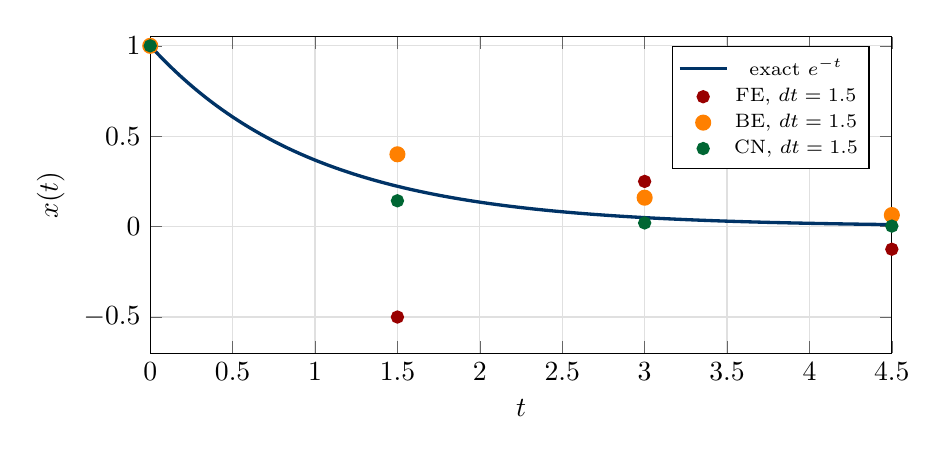
\begin{tikzpicture}
\begin{axis}[
    width=11cm, height=5.6cm,
    xlabel={$t$}, ylabel={$x(t)$},
    xmin=0, xmax=4.5, ymin=-0.7, ymax=1.05,
    legend pos=north east,
    legend style={font=\scriptsize, row sep=-1pt, inner sep=2pt},
    grid=both, grid style={gray!20},
    samples=200, domain=0:4.5,
    no markers
]
% Exact
\addplot[darkblue, very thick] {exp(-x)};
\addlegendentry{exact $e^{-t}$}

% lambda dt = 1.5, so N=8/3 ~ steps at multiples of 1.5 up to 4.5; use T=4.5, N=3
% Forward Euler: A = 1 - 1.5 = -0.5  -> 1, -0.5, 0.25, -0.125
\addplot[darkred, thick, mark=*, mark size=2pt, only marks]
  coordinates {(0,1) (1.5,-0.5) (3,0.25) (4.5,-0.125)};
\addlegendentry{FE, $dt=1.5$}

% Backward Euler: A = 1/(1+1.5) = 0.4 -> 1, 0.4, 0.16, 0.064
\addplot[orange, thick, mark=triangle*, mark size=2.5pt, only marks]
  coordinates {(0,1) (1.5,0.4) (3,0.16) (4.5,0.064)};
\addlegendentry{BE, $dt=1.5$}

% Crank-Nicolson: A = (1-0.75)/(1+0.75) = 1/7 ~ 0.1429 -> 1, 0.1429, 0.0204, 0.00292
\addplot[darkgreen, thick, mark=square*, mark size=2pt, only marks]
  coordinates {(0,1) (1.5,0.1429) (3,0.0204) (4.5,0.00292)};
\addlegendentry{CN, $dt=1.5$}

\end{axis}
\end{tikzpicture}
\end{center}

$\lambda=1$, $T=4.5$, $x_0=1$, $N=3$ ($\lambda dt = 1.5$). FE oscillates
around zero (since $1<\lambda dt<2$ gives $A<0$); BE overestimates the
decay (always positive but biased upwards); CN already underestimates
because $\lambda dt$ is large. All three fail visibly on a coarse grid,
each in its own way.

\end{frame}

\begin{frame}{Example -- Numerical comparison (refined grid)}

\begin{center}
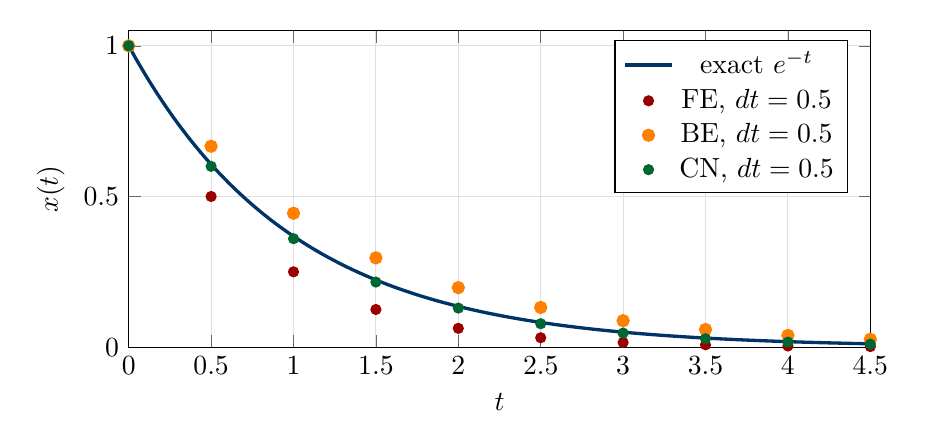
\begin{tikzpicture}
\begin{axis}[
    width=11cm, height=5.6cm,
    xlabel={$t$}, ylabel={$x(t)$},
    xmin=0, xmax=4.5, ymin=0, ymax=1.05,
    legend pos=north east,
    grid=both, grid style={gray!20},
    samples=200, domain=0:4.5,
    no markers
]
% Exact
\addplot[darkblue, very thick] {exp(-x)};
\addlegendentry{exact $e^{-t}$}

% dt = 0.5, lambda*dt = 0.5
% FE: A = 1 - 0.5 = 0.5, samples at 0,0.5,1,...,4.5: 0.5^k for k=0..9
\addplot[darkred, thick, mark=*, mark size=1.6pt, only marks, samples at={0,0.5,1,1.5,2,2.5,3,3.5,4,4.5}]
  {0.5^(2*x)};
\addlegendentry{FE, $dt=0.5$}

% BE: A = 1/1.5 = 2/3
\addplot[orange, thick, mark=triangle*, mark size=2pt, only marks, samples at={0,0.5,1,1.5,2,2.5,3,3.5,4,4.5}]
  {(2/3)^(2*x)};
\addlegendentry{BE, $dt=0.5$}

% CN: A = (1-0.25)/(1+0.25) = 0.6
\addplot[darkgreen, thick, mark=square*, mark size=1.6pt, only marks, samples at={0,0.5,1,1.5,2,2.5,3,3.5,4,4.5}]
  {0.6^(2*x)};
\addlegendentry{CN, $dt=0.5$}

\end{axis}
\end{tikzpicture}
\end{center}

Same problem, refined to $dt=0.5$ ($\lambda dt = 0.5$). FE now decays
monotonically but stays too low; BE stays too high; CN is visually on
top of the exact curve. Halving $dt$ divides CN's error by four
($O(dt^2)$) and the Eulers' by two ($O(dt)$).

\end{frame}

\begin{frame}{Nonlinear example -- Solow growth and its closed form}

\begin{itemize}

\item A genuinely \emph{nonlinear} state equation that still has an
  exact solution: the Solow growth model
  \[
  \dot k \;=\; s\,k^{\alpha} - \delta k,
  \qquad 0<\alpha<1,
  \]
  $s$ the saving rate, $\delta$ depreciation. One state ($k$), no jump
  — same boundary structure as the linear example, but the concave
  term $k^\alpha$ makes it nonlinear.

\item \textbf{Bernoulli trick.} Substitute $z = k^{1-\alpha}$:
  $\dot z = (1-\alpha)k^{-\alpha}\dot k = (1-\alpha)\bigl(s-\delta z\bigr)$
  — a \emph{linear} ODE. Hence the exact path
  \[
  k(t) = \Bigl[\tfrac{s}{\delta}
    + \bigl(k_0^{1-\alpha} - \tfrac{s}{\delta}\bigr)\,
      e^{-(1-\alpha)\delta\, t}\Bigr]^{\frac{1}{1-\alpha}}.
  \]

\item \textbf{Steady state and speed.} $k^\star=(s/\delta)^{1/(1-\alpha)}$,
  approached at rate $(1-\alpha)\delta$ — exactly the local eigenvalue
  $g'(k^\star)=s\alpha(k^\star)^{\alpha-1}-\delta=-(1-\alpha)\delta$. The
  Bernoulli map linearises the dynamics \emph{globally}, so local and
  global convergence rates coincide.

\item An exact yardstick on a nonlinear problem: only the scheme is
  approximated, never the truth.

\end{itemize}

\end{frame}

\begin{frame}{Nonlinear example -- Crank--Nicolson vs.\ the closed form}

\begin{itemize}

\item Implicit-midpoint residual with $g(k)=s\,k^\alpha-\delta k$:
  $\dfrac{k_{i+1}-k_i}{dt} = g\!\left(\dfrac{k_i+k_{i+1}}{2}\right)$.
  $g$ nonlinear, so each step is a scalar \emph{nonlinear} equation in
  $k_{i+1}$, solved by Newton — a 1-D preview of the stacked solve.

\end{itemize}

\vspace{-0.5ex}
\begin{center}
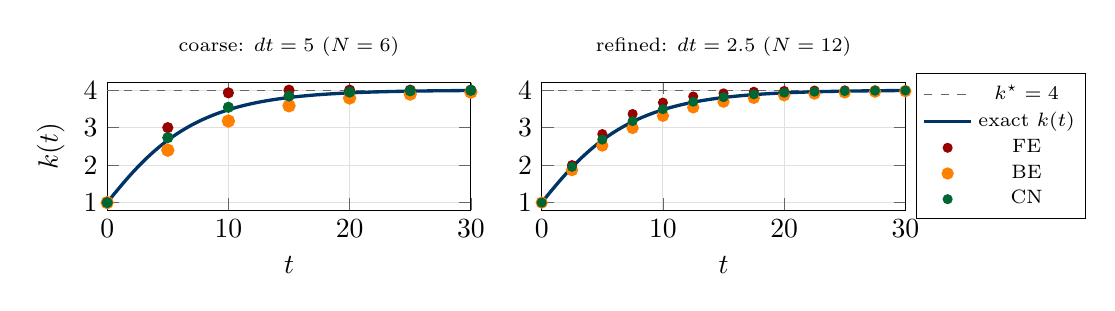
\begin{tikzpicture}
% --- coarse grid: dt = 5, N = 6 ---
\begin{axis}[
    name=coarse,
    width=6.2cm, height=3.2cm,
    title={\scriptsize coarse: $dt=5$ ($N=6$)},
    xlabel={$t$}, ylabel={$k(t)$},
    xmin=0, xmax=30, ymin=0.8, ymax=4.2,
    grid=both, grid style={gray!20},
    samples=200, domain=0:30,
    no markers
]
\addplot[gray, dashed] {4};
\addplot[darkblue, very thick] {(2 - exp(-0.2*x))^2};
\addplot[darkred, thick, mark=*, mark size=1.6pt, only marks]
  coordinates {(0,1)(5,3.0000)(10,3.9282)(15,3.9997)(20,4.0000)(25,4.0000)(30,4.0000)};
\addplot[orange, thick, mark=triangle*, mark size=2pt, only marks]
  coordinates {(0,1)(5,2.3981)(10,3.1753)(15,3.5819)(20,3.7895)(25,3.8944)(30,3.9471)};
\addplot[darkgreen, thick, mark=square*, mark size=1.6pt, only marks]
  coordinates {(0,1)(5,2.7321)(10,3.5425)(15,3.8434)(20,3.9473)(25,3.9824)(30,3.9941)};
\end{axis}
% --- refined grid: dt = 2.5, N = 12 ---
\begin{axis}[
    at={($(coarse.east)+(0.9cm,0)$)}, anchor=west,
    width=6.2cm, height=3.2cm,
    title={\scriptsize refined: $dt=2.5$ ($N=12$)},
    xlabel={$t$}, ylabel={},
    xmin=0, xmax=30, ymin=0.8, ymax=4.2,
    legend style={at={(1.03,0.5)}, anchor=west,
                  font=\scriptsize, row sep=-1pt, inner sep=2pt},
    grid=both, grid style={gray!20},
    samples=200, domain=0:30,
    no markers
]
\addplot[gray, dashed] {4};
\addlegendentry{$k^\star=4$}
\addplot[darkblue, very thick] {(2 - exp(-0.2*x))^2};
\addlegendentry{exact $k(t)$}
\addplot[darkred, thick, mark=*, mark size=1.4pt, only marks]
  coordinates {(0,1)(2.5,2.0000)(5,2.8284)(7.5,3.3636)(10,3.6680)(12.5,3.8304)(15,3.9143)(17.5,3.9569)(20,3.9784)(22.5,3.9892)(25,3.9946)(27.5,3.9973)(30,3.9986)};
\addlegendentry{FE}
\addplot[orange, thick, mark=triangle*, mark size=1.8pt, only marks]
  coordinates {(0,1)(2.5,1.8660)(5,2.5207)(7.5,2.9893)(10,3.3155)(12.5,3.5390)(15,3.6906)(17.5,3.7928)(20,3.8615)(22.5,3.9075)(25,3.9382)(27.5,3.9588)(30,3.9725)};
\addlegendentry{BE}
\addplot[darkgreen, thick, mark=square*, mark size=1.4pt, only marks]
  coordinates {(0,1)(2.5,1.9537)(5,2.6809)(7.5,3.1752)(10,3.4930)(12.5,3.6914)(15,3.8133)(17.5,3.8874)(20,3.9322)(22.5,3.9593)(25,3.9755)(27.5,3.9853)(30,3.9912)};
\addlegendentry{CN}
\end{axis}
\end{tikzpicture}
\end{center}

{\small\sloppy $\alpha=\tfrac12$, $s=0.8$, $\delta=0.4$ ($k^\star=4$),
$k_0=1$, $T=30$. Coarse grid magnifies the split (FE over, BE under, CN
closest); halving $dt$ divides CN's max error by four ($0.068\to0.018$) —
\textbf{second order survives}.\par}

\end{frame}

%==============================================================================
\section{The stacked system}
%==============================================================================

\begin{frame}{Stacked system -- Dynamic vs.\ algebraic rows}

\begin{itemize}

\item Of the $n$ rows of $F$, only the $n_d$ \textbf{dynamic} rows
  involve $\dot x$. Crank--Nicolson collocates these on each interval
  ($N$ blocks). (The dynamic \emph{variables} fill the first $n_d$
  columns -- states then jumps -- so $\dot x$ hits a contiguous block;
  the rows themselves may sit in any order.)\newline

\item The $n_a$ \textbf{algebraic} rows have $\dot x$ absent: there is
  nothing to discretise. They are enforced \textbf{pointwise} at every
  grid point ($N{+}1$ blocks).\newline

\item Equation count, matching the $n(N{+}1)$ unknowns exactly:
  \medskip
  \begin{center}
    \scriptsize
    \renewcommand{\arraystretch}{1.15}
    \begin{tabular}{lcc}
      \toprule
      Source & Per slot & Count \\
      \midrule
      Dynamic rows (CN collocation) & $n_d$ & $N\cdot n_d$ \\
      Algebraic rows (pointwise) & $n_a$ & $(N{+}1)\cdot n_a$ \\
      Initial states & $1$ & $n_S$ \\
      Terminal jumps & $1$ & $n_J$ \\
      \midrule
      \textbf{Total} & & $n(N{+}1)$ \\
      \bottomrule
    \end{tabular}
  \end{center}

\end{itemize}

\end{frame}

\begin{frame}{Stacked system -- Assembly}

\begin{itemize}

\item Stack the unknowns $X = (x_0,\ldots,x_N) \in \mathbb R^{n(N+1)}$ and
  assemble the residual $G(X)$ by stacking four row-groups,
  \emph{in this order}:\newline
  \begin{enumerate}
  \item dynamic rows of $R_i(x_i,x_{i+1})$, for $i=0,\ldots,N-1$
    \hfill ($N$ blocks of $n_d$);\newline
  \item algebraic rows of $F$ at every grid point
    \hfill ($N{+}1$ blocks of $n_a$);\newline
  \item initial-condition equations $x_{0,s} - x_s^0$ for each state
    \hfill ($n_S$ scalars);\newline
  \item terminal-condition equations $x_{N,j} - \bar x_j$ for each jump
    \hfill ($n_J$ scalars).\newline
  \end{enumerate}

\item Total: $n(N{+}1)$ equations in $n(N{+}1)$ unknowns. The
  assembly is symbolic (CasADi), so the Jacobian comes for free with
  \texttt{ca.jacobian(g, X)} —\;exact, sparse, and machine-precision.

\end{itemize}

\end{frame}

\begin{frame}{Stacked system -- Sparsity pattern of $J = \partial G/\partial X$}

\begin{center}
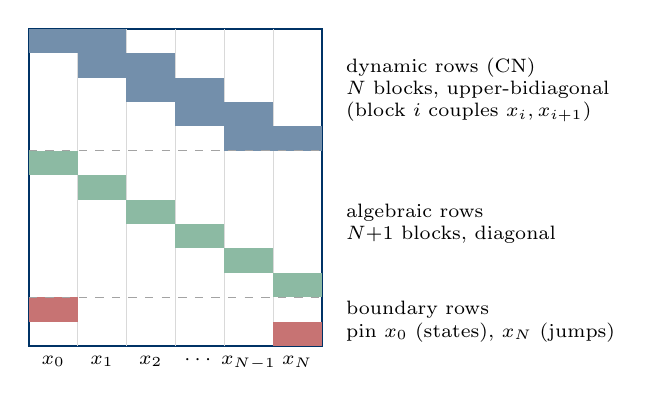
\begin{tikzpicture}[scale=0.62]
  % Rows are stacked in three contiguous groups (cf. previous slide):
  %   dynamic CN rows (N=5 blocks), then algebraic rows (N+1=6 blocks),
  %   then the two boundary rows. Columns are the grid blocks x_0 .. x_N.
  % cell width 1, cell height 0.5; total height H = 13*0.5 = 6.5.

  % outer box
  \draw[thick,darkblue] (0,0) rectangle (6,6.5);

  % faint column separators
  \foreach \c in {1,2,3,4,5} { \draw[gray!25,very thin] (\c,0) -- (\c,6.5); }

  % --- dynamic stripe: rows i=0..N-1, block-row i hits columns x_i, x_{i+1}
  \foreach \i in {0,1,2,3,4} {
    \fill[darkblue!55] (\i,{6.0-0.5*\i})  rectangle (\i+1,{6.5-0.5*\i});
    \fill[darkblue!55] (\i+1,{6.0-0.5*\i}) rectangle (\i+2,{6.5-0.5*\i});
  }

  % --- algebraic stripe: rows j=0..N, diagonal (column x_j only)
  \foreach \j in {0,1,2,3,4,5} {
    \fill[darkgreen!45] (\j,{3.5-0.5*\j}) rectangle (\j+1,{4.0-0.5*\j});
  }

  % --- boundary rows: initial states pin x_0, terminal jumps pin x_N
  \fill[darkred!55] (0,0.5) rectangle (1,1.0);   % initial states  -> column x_0
  \fill[darkred!55] (5,0.0) rectangle (6,0.5);   % terminal jumps  -> column x_N

  % stripe separators
  \draw[gray!60,dashed] (0,4.0) -- (6,4.0);
  \draw[gray!60,dashed] (0,1.0) -- (6,1.0);

  % column labels
  \node[below,font=\scriptsize] at (0.5,0) {$x_0$};
  \node[below,font=\scriptsize] at (1.5,0) {$x_1$};
  \node[below,font=\scriptsize] at (2.5,0) {$x_2$};
  \node[below,font=\scriptsize] at (3.5,0) {$\cdots$};
  \node[below,font=\scriptsize] at (4.5,0) {$x_{N-1}$};
  \node[below,font=\scriptsize] at (5.5,0) {$x_N$};

  % stripe labels (right)
  \node[right,align=left,font=\scriptsize] at (6.3,5.25)
    {dynamic rows (CN)\\$N$ blocks, upper-bidiagonal\\(block $i$ couples $x_i,x_{i+1}$)};
  \node[right,align=left,font=\scriptsize] at (6.3,2.5)
    {algebraic rows\\$N{+}1$ blocks, diagonal};
  \node[right,align=left,font=\scriptsize] at (6.3,0.5)
    {boundary rows\\pin $x_0$ (states), $x_N$ (jumps)};
\end{tikzpicture}
\end{center}

Grouping the rows as on the previous slide — the $N$ dynamic CN blocks
first, then the $N{+}1$ algebraic blocks, then the two boundary rows —
$J$ is \textbf{not} a single banded matrix: an upper-bidiagonal dynamic
stripe (block-row $i$ touches $x_i,x_{i+1}$) on top of a diagonal
algebraic stripe, closed by boundary entries pinning $x_0,x_N$.
Non-zeros $O(n^2 N)$. The two-point coupling makes $J$
\textbf{block-triangular} after a permutation — KLU\,+\,BTF resolves it in a
single sweep (next slides), keeping the solve linear in $N$.

\end{frame}

\begin{frame}{Stacked system -- Newton}

\begin{itemize}

\item At iterate $X^{(k)}$, solve the sparse linear system
  \[
  J\bigl(X^{(k)}\bigr)\,\Delta X \;=\; -\,G\bigl(X^{(k)}\bigr),
  \]
  then update $X^{(k+1)} = X^{(k)} + \alpha\,\Delta X$ with a
  step $\alpha\in(0,1]$.\newline

\item In Continuo: a \textbf{pluggable} sparse solver (default
  \texttt{klu}+BTF, SuperLU fallback — see next slides), a CasADi-supplied
  exact sparse Jacobian, $\|G\|_\infty$ convergence criterion ($10^{-10}$),
  max 50 iterations.\newline

\item A simple \textbf{backtracking line search} halves $\alpha$ until
  $\|G(X^{(k+1)})\|_\infty < \|G(X^{(k)})\|_\infty$, which prevents
  pure-Newton overshoots far from the solution.\newline

\item \textbf{Initial guess.} Default: the terminal steady state
  replicated at every grid point. For mildly non-linear models this is
  enough; for harder problems one can warm-start from a coarser grid
  or from a homotopy.

\end{itemize}

\end{frame}

\begin{frame}{Stacked system -- The linear core}

\begin{itemize}

\item Every Newton step solves one sparse system $J\,\Delta X = -G$. The
  \textbf{sparsity pattern of $J$ is constant} — across Newton iterations,
  and (at a fixed grid) across the segments of a multi-segment run.\newline

\item So the \textbf{symbolic} work (fill-reducing ordering, block structure)
  is done \emph{once} and only the \textbf{numeric} factorisation is
  refreshed. Continuo exposes this as a pluggable interface,
  \[
  \texttt{analyze} \;\to\; \texttt{factor} \;\to\; \texttt{refactor}
  \;\to\; \texttt{solve},
  \]
  with \texttt{analyze} hoisted out of the loop, so each step is just
  \texttt{refactor + solve}.\newline

\item Backends: \texttt{superlu} (SciPy, always available — the fallback),
  \texttt{klu} (SuiteSparse, the \textbf{default}), \texttt{umfpack},
  \texttt{pardiso}; selected by \texttt{auto} unless pinned.

\end{itemize}

\end{frame}

\begin{frame}{Stacked system -- Block-triangular form (BTF)}

\begin{center}
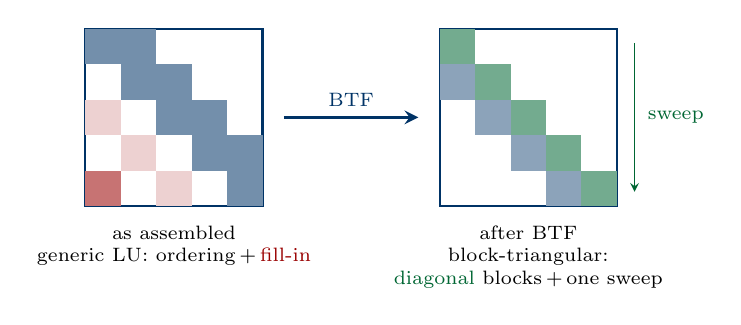
\begin{tikzpicture}[scale=0.9]
  % --- LEFT: J as assembled, seen as a generic sparse matrix ------------
  \draw[thick,darkblue] (0,0) rectangle (2.5,2.5);
  % diagonal (blue)
  \fill[darkblue!55] (0,2) rectangle (0.5,2.5);
  \fill[darkblue!55] (0.5,1.5) rectangle (1,2);
  \fill[darkblue!55] (1,1) rectangle (1.5,1.5);
  \fill[darkblue!55] (1.5,0.5) rectangle (2,1);
  \fill[darkblue!55] (2,0) rectangle (2.5,0.5);
  % super-diagonal (blue) -- CN couples x_i, x_{i+1}
  \fill[darkblue!55] (0.5,2) rectangle (1,2.5);
  \fill[darkblue!55] (1,1.5) rectangle (1.5,2);
  \fill[darkblue!55] (1.5,1) rectangle (2,1.5);
  \fill[darkblue!55] (2,0.5) rectangle (2.5,1);
  % boundary entry, below the diagonal (red)
  \fill[darkred!55] (0,0) rectangle (0.5,0.5);
  % fill-in a generic LU would create (faded red)
  \fill[darkred!18] (0,1) rectangle (0.5,1.5);
  \fill[darkred!18] (0.5,0.5) rectangle (1,1);
  \fill[darkred!18] (1,0) rectangle (1.5,0.5);
  \node[below,align=center,font=\scriptsize] at (1.25,-0.15)
    {as assembled\\generic LU: ordering\,+\,\textcolor{darkred}{fill-in}};

  % --- arrow ------------------------------------------------------------
  \draw[->,>=stealth,very thick,darkblue] (2.8,1.25) -- (4.7,1.25)
    node[midway,above,font=\scriptsize]{BTF};

  % --- RIGHT: after BTF, block lower-triangular -------------------------
  \draw[thick,darkblue] (5,0) rectangle (7.5,2.5);
  % diagonal blocks (green) -- the only ones LU-factorised
  \fill[darkgreen!55] (5,2) rectangle (5.5,2.5);
  \fill[darkgreen!55] (5.5,1.5) rectangle (6,2);
  \fill[darkgreen!55] (6,1) rectangle (6.5,1.5);
  \fill[darkgreen!55] (6.5,0.5) rectangle (7,1);
  \fill[darkgreen!55] (7,0) rectangle (7.5,0.5);
  % sub-diagonal coupling (blue) -- resolved by substitution
  \fill[darkblue!45] (5,1.5) rectangle (5.5,2);
  \fill[darkblue!45] (5.5,1) rectangle (6,1.5);
  \fill[darkblue!45] (6,0.5) rectangle (6.5,1);
  \fill[darkblue!45] (6.5,0) rectangle (7,0.5);
  \draw[->,>=stealth,darkgreen] (7.75,2.3) -- (7.75,0.2);
  \node[right,font=\scriptsize,darkgreen] at (7.8,1.25){sweep};
  \node[below,align=center,font=\scriptsize] at (6.25,-0.15)
    {after BTF\\block-triangular:\\\textcolor{darkgreen}{diagonal} blocks\,+\,one sweep};
\end{tikzpicture}
\end{center}

\begin{itemize}

\item The two-point CN stencil couples only neighbours $(x_i,x_{i+1})$, and
  the boundary data is \textbf{split} ($x_0$ states, $x_N$ jumps). The
  dependency graph is therefore \textbf{acyclic}: $J$ permutes to
  \textbf{block-triangular} form.\newline

\item \textbf{BTF} (a maximum transversal plus strongly-connected components)
  finds that permutation automatically; KLU then LU-factorises only the small
  $n\times n$ \textbf{diagonal blocks} and resolves the coupling by
  \textbf{back-substitution} — one sweep, with \emph{no fill}.

\end{itemize}

\end{frame}

\begin{frame}{Stacked system -- Why KLU+BTF here}

A generic sparse LU (SuperLU, UMFPACK) ignores this structure: it pays for a
fill-reducing ordering and a full factorisation. On the real example
Jacobians, the warm per-iteration solve (\texttt{refactor+solve}) is about
\textbf{$7\times$ faster} with KLU\,+\,BTF:

\begin{center}
\small
\renewcommand{\arraystretch}{1.2}
\begin{tabular}{lccc}
  \toprule
  model ($n$) & SuperLU & KLU\,+\,BTF & speed-up \\
  \midrule
  rbc ($1004$)          & $281$ & $39$  & $7.2\times$ \\
  nk-nonlinear ($3005$) & $463$ & $62$  & $7.5\times$ \\
  goodwin ($4802$)      & $830$ & $107$ & $7.8\times$ \\
  \bottomrule
\end{tabular}
\end{center}
\centerline{\scriptsize $\mu$s; UMFPACK $\approx$ SuperLU, PARDISO far slower at this $K$.}

\medskip

\begin{itemize}

\item \textbf{Why ``in this context''?} BTF wins because Crank--Nicolson is a
  \textbf{one-step} scheme. A \textbf{multi-step} scheme (BDF, 3-point — like
  Dynare) gives a \emph{banded but not triangular} Jacobian: BTF buys nothing
  (and can even slow it down), and a \textbf{banded} solver is the right tool.
  Hence the pluggable interface, with \texttt{auto} routing by the scheme's
  stencil: one-step $\to$ KLU\,+\,BTF, multi-step $\to$ banded.

\end{itemize}

\end{frame}

\begin{frame}{Stacked system -- Anticipated vs.\ surprise shocks}

\begin{itemize}

\item Within a single \textbf{information segment}, all future
  exogenous values are known: $e(t)$ is just a deterministic function
  evaluated at the midpoints.\newline

\item A \textbf{surprise} corresponds to a change in the information
  set at some reveal time $t_r$. Continuo's orchestrator
  partitions $[0,T]$ into segments separated by reveal times and
  solves \emph{one} perfect-foresight problem per segment:
  \begin{itemize}
  \item the segment's grid extends a full horizon $T$ past $t_r$
    (agents believe the new beliefs hold forever),\newline
  \item the state at $t_r$ is carried from the previous
    segment (states cannot jump),\newline
  \item the jump variables re-optimise at $t_r$ given the new
    beliefs.
  \end{itemize}

\item Each segment uses the \emph{same} CN+Newton machinery — surprises
  are just a sequence of perfect-foresight solves, glued together.

\end{itemize}

\end{frame}

%==============================================================================
\section{Comparison with Dynare (discrete time models)}
%==============================================================================

\begin{frame}{Comparison -- Side by side}

\begin{center}
\scriptsize
\renewcommand{\arraystretch}{1.2}
\begin{tabular}{p{3.4cm}p{4.4cm}p{4.4cm}}
  \toprule
   & \textbf{Dynare} & \textbf{Continuo (Crank--Nicolson)} \\
  \midrule
  Model       & $f(y_{t+1},y_t,y_{t-1},u_t,\theta)=0$ &
                $F(\dot x, x, e, \theta, t)=0$ \\
  Time        & intrinsically discrete & continuous, discretised on a grid \\
  Step size   & $1$ period & free $dt = T/N$ \\
  Discr. error & none & $O(dt^2)$ globally \\
  Stencil per eqn. & 3 points ($t{-}1,t,t{+}1$) & 2 points ($t_i,t_{i+1}$) \\
  Jacobian & block tridiagonal & block bidiagonal + block diagonal \\
  Default solver & sparse direct (UMFPACK) & KLU\,+\,BTF (auto), SuperLU fallback \\
  Boundary data & $y_0$, $\bar y_{T+1}$ for all & $x_S(0)$, $\bar x_J(T)$ split by type \\
  Algebraic vars & like any equation & detected, enforced pointwise \\
  Symbolic engine & custom C preprocessor & CasADi (Python) \\
  \bottomrule
\end{tabular}
\end{center}

\end{frame}

\begin{frame}{Comparison -- Conceptual mapping}

\begin{itemize}

\item Both methods reduce the BVP to a square non-linear system
  solved by Newton on a stacked vector of unknowns. The skeleton is
  identical:
  \[
  G(X) = 0,
  \qquad
  X^{(k+1)} = X^{(k)} - \alpha\,J^{-1} G(X^{(k)}).
  \]

\item \textbf{Why does Dynare have a tridiagonal Jacobian but
  Continuo only a bidiagonal one?} Because Crank--Nicolson
  couples \emph{two} adjacent points; a discrete-time model can also
  reference $y_{t-1}$, coupling \emph{three}.\newline

\item \textbf{Could one use a 3-point scheme in continuous time?} Yes
  (BDF2, trapezoidal-BDF blends). It would buy higher accuracy or
  L-stability but reintroduce a tridiagonal pattern.\newline

\item Conversely, one can read Crank--Nicolson as a discrete-time
  Dynare model by treating $\tfrac12(x_i+x_{i+1})$ and
  $(x_{i+1}-x_i)/dt$ as new variables, the algebra is the same,
  the bookkeeping is just different.

\end{itemize}

\end{frame}

\begin{frame}{Comparison -- When does the difference matter?}

\begin{itemize}

\item \textbf{Step-size flexibility.} In Dynare $dt=1$ period is
  built in; refining requires reformulating the model at higher
  frequency. In Continuo $dt$ is a numerical knob: choose
  $N$ until $O(dt^2)$ accuracy is sufficient.\newline

\item \textbf{Calibration at the right frequency.} Continuous-time
  preferences and technologies are calibrated directly in flow units
  (rates per unit time). Discrete-time calibration must pick a
  convention (annual? quarterly?) and may suffer from time-aggregation
  bias for fast-moving variables.\newline

\item \textbf{Occasionally-binding constraints.} A constraint that
  binds for a short duration is naturally captured with a fine
  grid in continuous time; in discrete time the period length sets a
  lower bound on the resolution.\newline

\item \textbf{Symbolic differentiation.} Both pipelines need exact
  Jacobians. Continuo uses CasADi (operator overloading,
  automatic differentiation); Dynare uses a custom preprocessor that
  emits derivative code. Both are exact.

\end{itemize}

\end{frame}

%==============================================================================
\section{Conclusion}
%==============================================================================

\begin{frame}{Conclusion -- Take-aways}

\begin{itemize}

\item Solving a perfect-foresight model = solving a two-point BVP =
  stacking the unknowns at every time slot and running Newton on a
  square block-sparse non-linear system.\newline

\item \textbf{Crank--Nicolson} is the right default for
  continuous-time economic models: second-order accurate, A-stable,
  symmetric, only two points per stencil. It coincides with the
  implicit-midpoint rule on smooth solutions, which is the form
  Continuo uses internally.\newline

\item \textbf{Dynare} solves an analogous stacked Newton system but
  with an intrinsically discrete model, a 3-point stencil, and a sparse
  solve over its block-tridiagonal Jacobian.\newline

\item Both designs share the same backbone: \emph{symbolic Jacobian +
  sparse linear algebra + Newton}. The differences live in the
  pre-processing step (discretise an ODE \emph{vs.}\ accept a difference
  equation) and in how the resulting block structure is exploited.

\end{itemize}

\end{frame}

\begin{frame}{Conclusion -- Further reading}

\begin{itemize}

\item \textbf{Crank--Nicolson, BVPs and collocation.}  Ascher \&
  Petzold (1998), \emph{Computer Methods for Ordinary Differential
    Equations and Differential-Algebraic Equations}. Hairer \& Wanner
  (1996), \emph{Solving Ordinary Differential Equations II}. Iserles
  (2009), \emph{A First Course in the Numerical Analysis of
    Differential Equations}.\newline

\item \textbf{Dynare's algorithm.} Juillard (1996), \emph{Dynare:
    A program for the resolution and simulation of dynamic models with
    forward variables through the use of a relaxation algorithm},
  CEPREMAP. Adjemian \emph{et al.} (2026), \emph{Dynare Reference
    Manual}, Chap.\ ``Perfect-foresight simulation''.\newline

\end{itemize}

\end{frame}

\end{document}
